\documentclass[aspectratio=169,unicode,10pt]{beamer}
\usepackage{luatexja}
\usepackage[haranoaji]{luatexja-preset}
\usepackage{amsmath,amssymb,mathtools}
\usepackage{graphicx}
\usepackage{booktabs}
\usepackage{array}

\usetheme{default}
\usecolortheme{default}
\setbeamertemplate{navigation symbols}{}
\setbeamertemplate{footline}[frame number]
\setbeamerfont{frametitle}{size=\normalsize,series=\bfseries}
\setbeamerfont{title}{size=\large,series=\bfseries}

\graphicspath{{../final_report/figures/}}

\title{屋内 RSSI 位置推定の精度改善に向けた\\手法実装と評価}
\subtitle{最終発表}
\author{情報通信システム論 I\quad グループ [GROUP\_NAME]\\{[AUTHOR\_NAME]}}
\institute{}
\date{2026 年 7 月 24 日}

\begin{document}

\begin{frame}
  \titlepage
\end{frame}

\begin{frame}{背景と目的}
  \begin{itemize}
    \item 対象：豊橋技術科学大学 3F 廊下の WiFi (tutwifi/tutwifi2025) RSSI による屋内位置推定
    \item 公表ベースライン：\textbf{PBL 4.38 m / CLA 8.07 m / WCL 3.57 m}（往路平均誤差）\cite{blumenthal2007wcl,tanaka2023tut}
    \item WCL の限界：AP 群の凸包内に推定が閉じ込められ，重み設計の物理的根拠も弱い
    \item \textbf{目標：平均誤差 2 m 未満を達成する}
    \item 方針：公表ベースラインを生 RSSI から\emph{完全再現}して比較基準を凍結し，その上に 12 手法（Tier~1--3）を実装・評価
  \end{itemize}
\end{frame}

\begin{frame}{提案アプローチの全体像}
  \begin{itemize}
    \item \textbf{Tier 1：本命 fingerprinting}\;
      wknn / gp\_corridor / studentt\_fp
    \item \textbf{Tier 2：相対化 fingerprinting}\;
      centered\_fp（オフセット除去）/ rank\_fp（順位変換）
    \item \textbf{Tier 3：WCL 改良系（アブレーション基準）}\;
      power-domain・linpower・top-$L$・blacklist・varweight・multiband・廊下射影
    \item \textbf{中核アイデア：\texttt{gp\_corridor}（廊下 1D の Gaussian Process radio map）}
      \begin{itemize}
        \item 廊下 arc-length $s$ 上で AP-band ごとに Matérn-3/2 GP を張る\cite{ferris2007gpslam}
        \item セグメント分類（C/C2/C3）$\to$ セグメント内 1D 尤度推定の階層構成
      \end{itemize}
  \end{itemize}
\end{frame}

\begin{frame}{手法：Tier 1（本命）}
  \small
  \begin{itemize}
    \item \textbf{wknn}\; RSSI ベクトルの逆距離加重 K 近傍。K・重みは inner-CV（$K{=}5$, inv\_sq）
    \item \textbf{gp\_corridor}\; 廊下 arc-length $s$ の Matérn-3/2 GP を (AP,band) 毎に張る（102 鍵中 82 鍵）
    \[
      k(s,s')=\sigma_f^2\Bigl(1+\tfrac{\sqrt{3}|s-s'|}{\ell}\Bigr)\exp\Bigl(-\tfrac{\sqrt{3}|s-s'|}{\ell}\Bigr)
    \]
    \item \textbf{studentt\_fp}\; Student-$t$ 尤度＋Bernoulli 検出項＋共通オフセット補正 $\hat\delta_q$（$\nu{=}3$ 選択）\cite{youssef2005horus}
  \end{itemize}
\end{frame}

\begin{frame}{手法：Tier 2--3}
  \small
  \textbf{Tier 2 — 相対化（scan 共通オフセット除去）}
  \begin{itemize}
    \item \textbf{centered\_fp}：$\tilde r_{s,a}=r_{s,a}-\operatorname*{median}_{j} r_{s,j}$，$\lambda{=}0.25$
    \item \textbf{rank\_fp}：RSSI 絶対値でなく AP 強度順位を用いる（加法オフセット不変）
  \end{itemize}
  \vspace{2pt}
  \textbf{Tier 3 — WCL 改良（凸包制約を保持したままの重み調整）}
  \begin{itemize}
    \item power-domain / linpower / top-$L$ / 廊下射影 / blacklist / varweight / multiband
    \item いずれも WCL の凸包制約という根本問題を持ち越すため，2~m 未満は達成不能と予想
  \end{itemize}
\end{frame}

\begin{frame}{評価プロトコル}
  \begin{itemize}
    \item \textbf{Protocol A}（2 fold）：往路で DB 構築 $\to$ 復路でテスト，およびその逆
      \begin{itemize}
        \item 同一 59 地点が train/test 双方に現れる $\Rightarrow$ 本質は\textbf{測量済み地点の再認識}
      \end{itemize}
    \item \textbf{LOLO}（Leave-One-Location-Out, 59 fold）：train = 往路 \textbackslash \{保持地点\}，test = \emph{復路}の当該地点
      \begin{itemize}
        \item 未測量地点 \textbf{かつ} 方向も異なる $\Rightarrow$ \textbf{空間汎化と方向汎化の同時テスト}
        \item 本研究の\textbf{決定的テスト}と位置付ける
      \end{itemize}
    \item \textbf{リーク対策}：分割 iterator で構造的に除外し，spy テストで検証
    \item \textbf{統計}：地点別誤差上の paired bootstrap ($B{=}1000$, seed$=$0) で 95\% CI
    \item ハイパーパラメータは train 内 5-fold inner-CV，GP のみ train 上の周辺尤度でグリッド選択
  \end{itemize}
\end{frame}

\begin{frame}{結果：LOLO（決定的テスト）}
  \centering\footnotesize
  \begin{tabular}{lrrrr}
    \toprule
    Method & Ave [m] & Median & P90 & $\leq$2m 率 \\
    \midrule
    \textbf{gp\_corridor} & \textbf{0.72} & \textbf{0.50} & \textbf{1.74} & \textbf{0.90} \\
    wknn                 & 2.07 & 1.34 & 4.15 & 0.71 \\
    centered\_fp         & 2.08 & 1.37 & 4.11 & 0.71 \\
    studentt\_fp         & 2.32 & 2.00 & 4.00 & 0.58 \\
    rank\_fp             & 2.70 & 1.35 & 3.88 & 0.76 \\
    \midrule
    wcl\_corridor (Tier 3 最良) & 3.31 & 2.77 & 6.00 & 0.41 \\
    wcl（ベースライン）  & 3.51 & 2.81 & 6.09 & 0.31 \\
    pbl                   & 4.52 & 3.67 & 7.98 & 0.24 \\
    cla                   & 7.02 & 6.53 & 12.41 & 0.12 \\
    \bottomrule
  \end{tabular}
  \vspace{6pt}
  \begin{itemize}\footnotesize
    \item \textbf{gp\_corridor が Ave 0.72 m，$\leq$2 m 率 90\%}で目標達成
    \item Tier 1/2 の 4 手法はいずれも WCL~3.51 を大幅改善
    \item Tier 3 は小幅（凸包制約が本質的限界）
  \end{itemize}
\end{frame}

\begin{frame}{結果：CDF とセグメント別誤差}
  \centering
  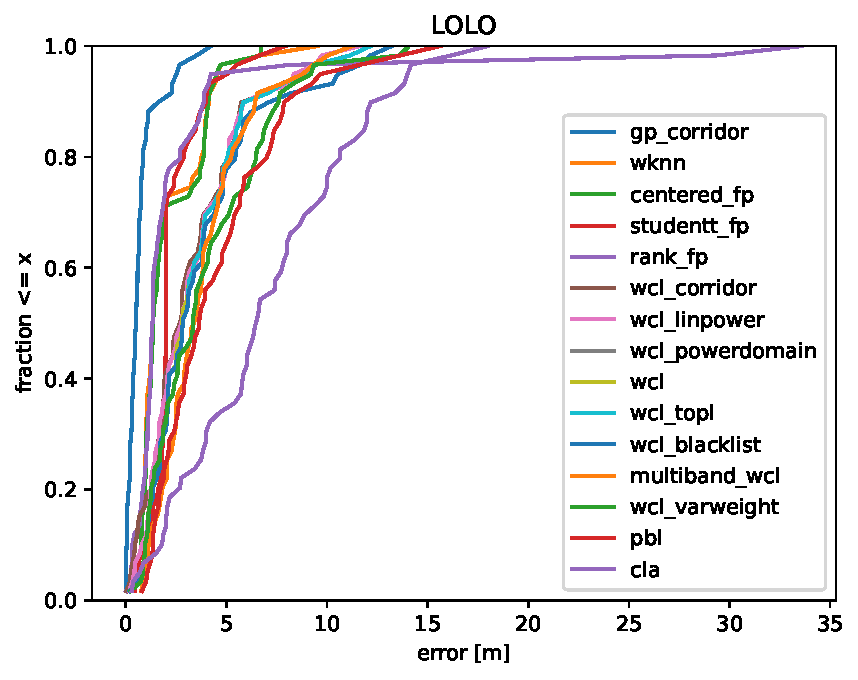
\includegraphics[width=0.42\linewidth]{cdf_lolo.pdf}\hfill
  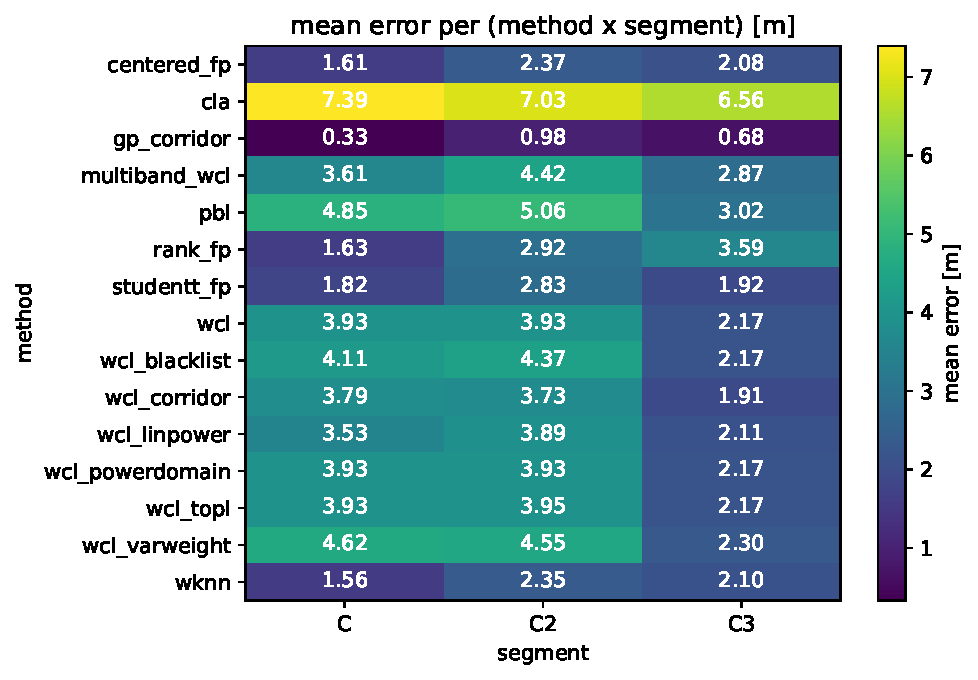
\includegraphics[width=0.56\linewidth]{segment_heatmap.pdf}
  \\[4pt]
  {\footnotesize 左：LOLO 誤差 CDF． 右：手法 $\times$ 廊下セグメントの平均誤差 [m]．}
\end{frame}

\begin{frame}{考察①：なぜ gp\_corridor が効いたか}
  \begin{itemize}
    \item 廊下が\textbf{1 次元多様体}であることを事前情報として明示的に利用
      \begin{itemize}
        \item 2D 座標 (x,y) ではなく arc-length $s$ で回帰 $\Rightarrow$ 有効自由度が大幅に減少
      \end{itemize}
    \item AP-band 毎に長さ尺度 $\ell$ を独立に学習 $\Rightarrow$ 空間的平滑性の異なる AP を個別扱い
    \item セグメント分類（C/C2/C3, train accuracy 1.00）が\textbf{L 字廊下の壁越し相関}を切る
    \item LOLO $<$ Protocol A の逆転（0.72 $<$ 1.01）
      \begin{itemize}
        \item 仮説：Protocol A では往復差（方向依存オフセット）に過適合，LOLO では平滑補間が復路とよく整合
        \item 断定はしない — リークは spy テストで否定済み
      \end{itemize}
  \end{itemize}
\end{frame}

\begin{frame}{考察②：目標達成の意義と限界}
  \textbf{意義}
  \begin{itemize}
    \item $\leq$2 m 率 90\%：実質的に「廊下上の 2 m メッシュを正しく当てる」水準
    \item WCL~3.57 m $\to$ 0.72 m は\textbf{約 5 倍の精度向上}
    \item WCL との差 $-2.61$ m は 95\% CI $[-3.27, -1.94]$ で\textbf{統計的に有意}
  \end{itemize}
  \vspace{4pt}
  \textbf{限界（本文§6）}
  \begin{itemize}
    \item データ規模：59 地点 $\times$ 2 方向の小規模データ
    \item 打ち切り観測は Bernoulli 検出モデルで代替
    \item C4F 系の追加データ（dataset\_r0701）は未評価
    \item 地点 bootstrap は空間相関を無視した\textbf{記述的 CI}
  \end{itemize}
\end{frame}

\begin{frame}{付録：Tier 4 の追補評価（本文凍結後）}
  \begin{itemize}
    \item 時間があったため Tier 4 の 7 手法（Mahalanobis / gp\_augmented / joint\_fp / fisher / PLS / ordinal / wcl\_residual）を追加実装
    \item 結果は本文成果物と\textbf{別系統に隔離}（\texttt{results/tier4/}, \texttt{tables/tier4\_*.tex}）
    \item \textbf{主要比較 vs gp\_corridor を事前指定}：7 手法\textbf{すべて有意に劣る}
      \begin{itemize}
        \item mahalanobis 1.77 m ($\Delta$gp\_corridor $+1.04$, 95\% CI $[0.69, 1.38]$)
        \item gp\_augmented 1.87 m ($+1.15$, $[0.83, 1.47]$)
      \end{itemize}
    \item WKNN 系 4 手法は vs WCL では有意改善 (2 m 前後)
    \item ordinal は 59 標本で閾値ロジットが不安定 $\to$ 有意に悪化
  \end{itemize}
\end{frame}

\begin{frame}{まとめと今後}
  \textbf{達成}
  \begin{itemize}
    \item 公表ベースライン (PBL/CLA/WCL) を生 RSSI から凍結再現
    \item \texttt{gp\_corridor} で LOLO 平均 \textbf{0.72 m}，$\leq$2 m 率 90\%\\目標 $<$2 m を大幅にクリア
    \item 12 (+7) 手法を統一プロトコル・inner-CV・bootstrap CI で公正比較
  \end{itemize}
  \textbf{今後}
  \begin{itemize}
    \item Tier 5（HMM/Viterbi の時系列手法）：「RSSI のみ」の主張との整合を要検討
    \item 大規模データ（C4F 追加，dataset\_r0701）での外部妥当性検証
    \item 端末実装（Android アプリ化）への移行\cite{tanaka2023tut}
  \end{itemize}
\end{frame}

\begin{frame}[allowframebreaks]{参考文献}
  \footnotesize
  \begin{thebibliography}{9}
    \bibitem{blumenthal2007wcl}
      J.~Blumenthal, R.~Grossmann, F.~Golatowski, and D.~Timmermann,
      ``Weighted Centroid Localization in Zigbee-Based Sensor Networks,''
      \emph{Proc. IEEE International Symposium on Intelligent Signal Processing}, pp.~1--6, Oct.~2007.
    \bibitem{tanaka2023tut}
      田中空斗, 足立裕基, 小松和暉, 宮路祐一, 上原秀幸,
      ``大学構内における Wi-Fi の受信信号強度とスマートフォンを用いた屋内位置推定システムの開発,''
      信学論 B, Vol.~J107-B, No.~3, pp.~209--217, Oct.~2023.
    \bibitem{bulusu2000gpsless}
      N.~Bulusu, J.~Heidemann, and D.~Estrin,
      ``GPS-Less Low-Cost Outdoor Localization for Very Small Devices,''
      \emph{IEEE Personal Communications}, Vol.~7, Issue~5, pp.~28--34, Oct.~2000.
    \bibitem{krumm2004nearme}
      J.~Krumm and K.~Hinckley,
      ``The NearMe Wireless Proximity Server,''
      \emph{Proc. the Sixth International Conference on Ubiquitous Computing (UbiComp~2004)}, pp.~283--300, 2004.
    \bibitem{hara2010statloc}
      原 晋介,
      ``位置推定における統計的推定理論,''
      \emph{IEICE Fundamentals Review}, Vol.~4, No.~1, pp.~32--38, Jul.~2010.
    \bibitem{youssef2005horus}
      M.~Youssef and A.~Agrawala,
      ``The Horus Location Determination System,''
      \emph{Proc. ACM MobiSys}, 2005.
    \bibitem{ferris2007gpslam}
      B.~Ferris, D.~Fox, and N.~Lawrence,
      ``WiFi-SLAM Using Gaussian Process Latent Variable Models,''
      \emph{Proc. IJCAI}, 2007.
  \end{thebibliography}
\end{frame}

\end{document}
